%%%% ANEXO B
%%
%% Texto ou documento não elaborado pelo autor, que serve de fundamentação, comprovação e ilustração.

%% Título e rótulo de anexo (rótulos não devem conter caracteres especiais, acentuados ou cedilha)
\chapter{Normas para elaboração de trabalhos acadêmicos}\label{cap:anexob}

As normas da \gls{utfpr} podem ser acessadas em: \url{http://portal.utfpr.edu.br/biblioteca/trabalhos-academicos/discentes/orientacao-para-trabalhos-academicos}. Ver Figura \ref{fig:capadolivro}.

\begin{figure}[htb]%% Ambiente figure
\captionsetup{width=0.9\textwidth}%% Largura da legenda
\caption{Sítio: Normas para Elaboração de Trabalhos Acadêmicos.}%% Legenda
\label{fig:capadolivro}%% Rótulo
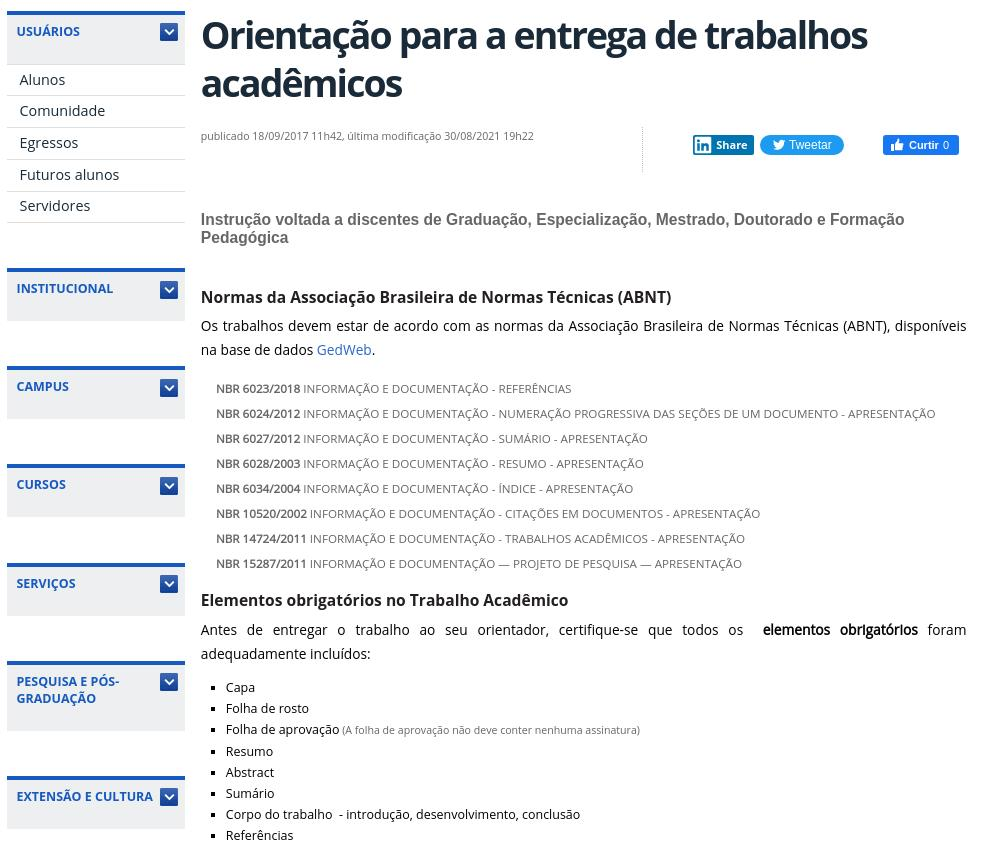
\includegraphics[width=0.9\textwidth]{normas}%% Dimensões e localização
\fonte{\cite{UTFPR2008}}%% Fonte
\end{figure}

